%%%%%%%%%%%%%%%%%%%%%%%%%%%%%%%%%%%%%%%%%%%%%%%%%%%%%%%%%%%%%%%%%%%%%%%%%%%%%%%%
% Version Control Systems
%
% Author: FOSSEE 
% Copyright (c) 2009, FOSSEE, IIT Bombay
%%%%%%%%%%%%%%%%%%%%%%%%%%%%%%%%%%%%%%%%%%%%%%%%%%%%%%%%%%%%%%%%%%%%%%%%%%%%%%%%

\documentclass[14pt,compress]{beamer}

\mode<presentation>
{
  \usetheme{Warsaw}
  \useoutertheme{infolines}
  \setbeamercovered{transparent}
}

\usepackage[english]{babel}
\usepackage[latin1]{inputenc}
%\usepackage{times}
\usepackage[T1]{fontenc}

% Taken from Fernando's slides.
\usepackage{ae,aecompl}
\usepackage{mathpazo,courier,euler}
\usepackage[scaled=.95]{helvet}

\definecolor{darkgreen}{rgb}{0,0.5,0}

\usepackage{listings}
\lstset{language=Python,
    basicstyle=\ttfamily\bfseries,
    commentstyle=\color{red}\itshape,
  stringstyle=\color{darkgreen},
  showstringspaces=false,
  keywordstyle=\color{blue}\bfseries}

%%%%%%%%%%%%%%%%%%%%%%%%%%%%%%%%%%%%%%%%%%%%%%%%%%%%%%%%%%%%%%%%%%%%%%
% Macros
\setbeamercolor{emphbar}{bg=blue!20, fg=black}
\newcommand{\emphbar}[1]
{\begin{beamercolorbox}[rounded=true]{emphbar} 
      {#1}
 \end{beamercolorbox}
}
\newcounter{time}
\setcounter{time}{0}
\newcommand{\inctime}[1]{\addtocounter{time}{#1}{\tiny \thetime\ m}}

\newcommand{\typ}[1]{\lstinline{#1}}

\newcommand{\kwrd}[1]{ \texttt{\textbf{\color{blue}{#1}}}  }

%%% This is from Fernando's setup.
% \usepackage{color}
% \definecolor{orange}{cmyk}{0,0.4,0.8,0.2}
% % Use and configure listings package for nicely formatted code
% \usepackage{listings}
% \lstset{
%    language=Python,
%    basicstyle=\small\ttfamily,
%    commentstyle=\ttfamily\color{blue},
%    stringstyle=\ttfamily\color{orange},
%    showstringspaces=false,
%    breaklines=true,
%    postbreak = \space\dots
% }

%%%%%%%%%%%%%%%%%%%%%%%%%%%%%%%%%%%%%%%%%%%%%%%%%%%%%%%%%%%%%%%%%%%%%%
% Title page
\title[Version Control Systems]{SEES: Version Control Systems}

\author[FOSSEE] {FOSSEE}

\institute[IIT Bombay] {Department of Aerospace Engineering\\IIT Bombay}
\date[]{}
%%%%%%%%%%%%%%%%%%%%%%%%%%%%%%%%%%%%%%%%%%%%%%%%%%%%%%%%%%%%%%%%%%%%%%

%\pgfdeclareimage[height=0.75cm]{iitmlogo}{iitmlogo}
%\logo{\pgfuseimage{iitmlogo}}


%% Delete this, if you do not want the table of contents to pop up at
%% the beginning of each subsection:
\AtBeginSubsection[]
{
  \begin{frame}<beamer>
    \frametitle{Outline}
    \tableofcontents[currentsection,currentsubsection]
  \end{frame}
}

\AtBeginSection[]
{
  \begin{frame}<beamer>
    \frametitle{Outline}
    \tableofcontents[currentsection,currentsubsection]
  \end{frame}
}

% If you wish to uncover everything in a step-wise fashion, uncomment
% the following command: 
%\beamerdefaultoverlayspecification{<+->}

%%\includeonlyframes{current,current1,current2,current3,current4,current5,current6}

%%%%%%%%%%%%%%%%%%%%%%%%%%%%%%%%%%%%%%%%%%%%%%%%%%%%%%%%%%%%%%%%%%%%%%
% DOCUMENT STARTS
\begin{document}

\begin{frame}
  \maketitle
\end{frame}

% CREATING TOC 
\begin{frame}
  \frametitle{Outline}
  \tableofcontents
  % You might wish to add the option [pausesections]
\end{frame}

%% There are some %$ used just to minimise the effect of $ sign used in lstlisting. In emacs it looks unhealthy.

% Introduction to course-need of version control, history, options available.
\section{Introduction}

%% Home made version control system?
\begin{frame}[fragile]
  \frametitle{Home-brew}
  \begin{center}
    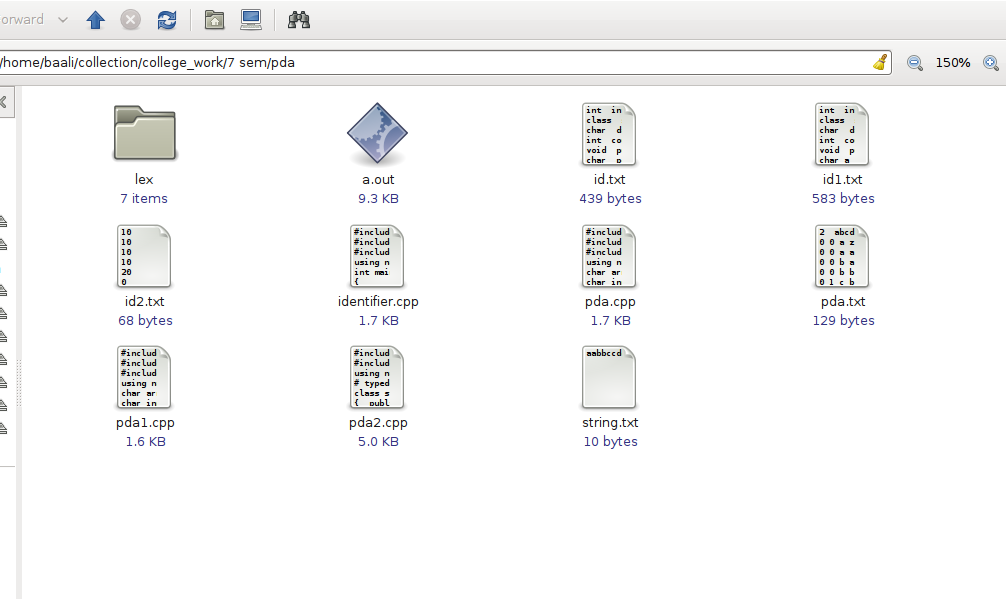
\includegraphics[height=1.8in,width=4.2in]{folder.png}
  \end{center}
  \begin{lstlisting}
$ ls
a.out  id1.txt  id2.txt  identifier.cpp  id.txt  lex  pda1.cpp  pda2.cpp  pda.cpp  pda.txt  string.txt
  \end{lstlisting} %%$
    %%a screen-shot of folder with all crazy names.  
\end{frame}

\begin{frame}[fragile]
  \frametitle{Problems with such nomenclature}  
  \begin{block}{}    
  \begin{itemize}
  \item Difficult to relate to content of file.
  \item Cant track changes done to file.
  \item It wont scale.
  \end{itemize}
    \end{block}
\end{frame}

\begin{frame}
  \frametitle{What is version control}
  \begin{block}{From a blog post}
    ``Version control (or source control) is nothing more than keeping copies of work as we make changes to it.''
  \end{block}
\end{frame}

\begin{frame}[fragile]
  \frametitle{Need of Version Control}
  \begin{itemize}
  \item Track the history and evolution of a program.
  \item To collaborate effectively on a project.
  \item \begin{color}{red}``To err is Human''\end{color} for recovery we have ...
  \end{itemize}
\end{frame}

%% Introduction to how logs are managed in VCS.
%% A analogy in logs and day-to-day life?
\begin{frame}[fragile]
  \frametitle{How does it work? Analogy}
  It can roughly be related to Computer/Video Games.
  \begin{itemize}
  \item We play games in stages.
  \item We pass a stage/task- \begin{color}{red}we SAVE the game.\end{color}
  \item We resume playing from there onwards.
  \item In-case we want to replay or revisit some particular stage, we start from position we saved earlier.
  \item Even we can change the course of play henceforth.
  \end{itemize}
\end{frame}

\begin{frame}[fragile]
  \frametitle{Better way to say:}
  \begin{center}
    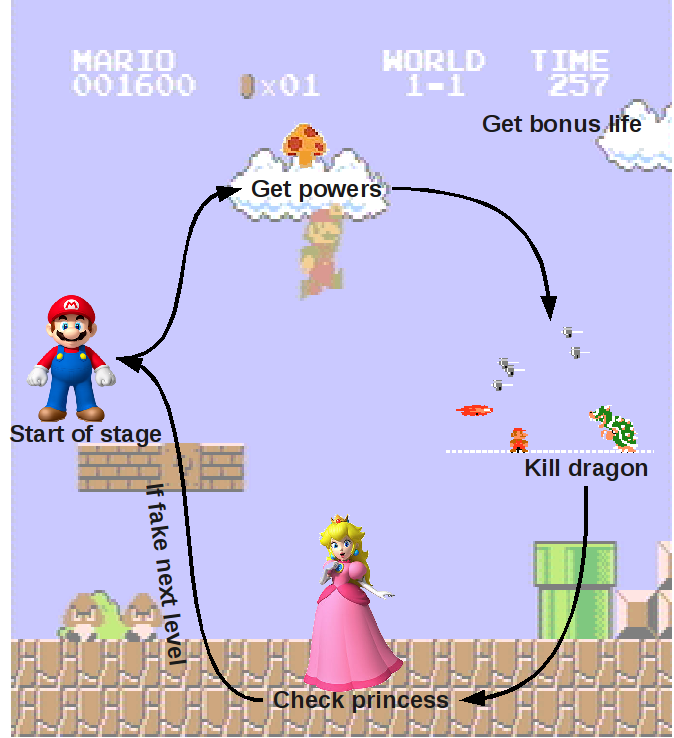
\includegraphics[height=2.5in,width=2.5in, interpolate=true]{mario}
  \end{center}  
  \emphbar{VCS provides power to save and resume from a stage.}
\end{frame}

\begin{frame}
  \frametitle{How is it done?}
  \begin{itemize}
  \item It keeps track of changes you make to a file. You can improve, revisit, and amend.
  \item All changes are logged/recorded, so you and others can follow the development cycle.
  \end{itemize}  
\end{frame}


%% Introduction to jargon 
%% This should have some excerpts from normal systems.
%% Like diffs, folders etc.

%% \section{Learning the Lingo!}

%% \begin{frame}[fragile]
%%   \frametitle{Common jargon: Basic setup}
%%   \begin{lstlisting}
%% $ ls slides/
%% filter.png  lena_mean.png  lena.png  
%% neighbour.png  pool.aux  pool.log  
%% pool.nav  pool.out  pool.pdf  pool.snm  
%% pool.tex  pool.tex~  pool.toc  pool.vrb    
%%   \end{lstlisting}  %%$
%%   \begin{itemize}
%%   \item Repository(repo):\\
%%         The folder with all files.
%%   %% \item Server:\\
%%   %%       Machine with main inventory/repo.
%%   %% \item Client:\\
%%   %%       Local machines with copy of main repo.
%%   \end{itemize}
%% \end{frame}

%% \begin{frame}[fragile]
%%   \frametitle{Actions}
%%   \begin{itemize}
%%   \item Add:\\
%%     Creating/Copying files(cp, touch).
%%   \item Check out/Clone:\\
%%     Creating copy of working folder.
%%   \end{itemize}
%%   \begin{lstlisting}
%% $ cp -rv circulate/ local
%% `circulate/' -> `local'
%% `circulate/sslc1.txt' -> `local/sslc1.txt'
%% `circulate/pos.txt' -> `local/pos.txt'
%% `circulate/pendulum.txt' -> `local/pendulum.txt'
%% `circulate/lena.png' -> `local/lena.png'
%% `circulate/sslc1.py' -> `local/sslc1.py'
%% `circulate/points.txt' -> `local/points.txt'    
%%   \end{lstlisting}  %%$
%% \end{frame}

%% \begin{frame}
%%   \frametitle{Actions cont...}
%%   \begin{itemize}
%%     \item Version:\\
%%     Version number(Die Hard 4.0).\\
%%     Making changes to folder, changes state/version.
%%     \item Head/Tip:\\
%%     Most recent revision/stage.
%%     \item Commit:\\
%%     Saving(recording) a change.
%%   \item Change log/History:\\
%%     List of all past changes.
%%   \end{itemize}
%% \end{frame}

%% \begin{frame}
%%   \frametitle{Actions cont...}
%%   \begin{itemize}
%%   \item Branch:\\
%%     Separate local copy for bug fixing, testing.
%%   \item Diff/Change:\\
%%     Changes made in a file in two different versions.
%%   \item Merge (or patch):\\
%%     Appling the changes to file, to make it up-to-date.
%%   \item Conflict:\\
%%     When merging a file is not obvious.
%%   \item Resolve:\\
%%     Fixing the conflict manually.
%%   \end{itemize}
%% \end{frame}

%% % Types of Version Controls
%% %% \section{Types of VCS}

%% %% \begin{frame}
%% %%   \frametitle{Types:}
%% %%   Based on ways of managing the repo there are two types of VCS:
%% %%   \begin{itemize}
%% %%   \item Centralized VCS\\
%% %%     cvs, svn fall under this category.
%% %%   \item Distributed VCS\\
%% %%     hg, bzr, git follows this methodology.
%% %%   \end{itemize}
%% %%   \emphbar{We would be covering \typ{hg}}
%% %% \end{frame}

\begin{frame}
  \frametitle{We will cover hg?}
    
\includegraphics[height=.75in, interpolate=true]{mercurial}\\
  Because it is:
  \begin{itemize}
  \item Easy to learn and use.
  \item Lightweight.
  \item Scales excellently.
  \item Written in Python.
  \end{itemize}
  \inctime{15}
\end{frame}

% Initializing the repo, cloning, committing changes, pushing, pulling to repo.
\section{Getting Started}

\begin{frame}
  \frametitle{Objective}
  \begin{block}{}
    We would \alert{manage} letters collaboratively using \typ{hg}.
  \end{block}

  %% \pause
  %% \begin{block}{Disclaimer}
  %%   Please note, objective is not to learn creative writing, but to learn \alert{hg(mercurial)} via \alert{interesting} use case.
  %% \end{block}    
\end{frame}

\begin{frame}[fragile]
  \frametitle{Getting comfortable:}
  For checking \typ{hg} installation and its version type:
  \begin{lstlisting}
    $ hg version    
  \end{lstlisting}
  To get broad help on \typ{hg} and commands available:
  \begin{lstlisting}
    $ man hg
    $ hg help
  \end{lstlisting}
  To get help on particular \typ{hg} related option try:
  \begin{lstlisting}
    $ hg help diff
  \end{lstlisting} %$
\end{frame}

\begin{frame}[fragile]
  \frametitle{Getting working/existing code base}
  To get a already existing code-base:
  \begin{lstlisting}
$ hg clone 
http://hg.serpentine.com/tutorial/hello 
localCopyhello
  \end{lstlisting}
\typ{localCopyhello} is copy of code-base. 
  \begin{lstlisting}
$ ls localCopyhello/
hello.c  Makefile
  \end{lstlisting}
\end{frame}

%%introduction to clone, repo, server, client.
\begin{frame}[fragile]
  \frametitle{What did we do!}
  \begin{block}{Explanation}
    \begin{itemize}
    \item<1-> \typ{hello} is a \alert{repo}, it's a collection of files and folders. 
    \item<2-> This repo is located on remote(\alert{server}) machine.    
    \item<3-> We copy(\alert{clone}) repo to our local machine.
    \end{itemize}    
  \end{block}
\end{frame}

\begin{frame}[fragile]
  \frametitle{Creating repo of existing files}
  I have some files which I want to bring under version control. \typ{hg} provides \alert{\typ{init}} command for this: 
  \begin{lstlisting}
$ ls -a circulate/
.  ..  lena.png  pendulum.txt  points.txt  pos.txt  sslc1.py  sslc1.txt
$ cd circulate/
$ hg init
$ ls -a
.  ..  .hg  lena.png  pendulum.txt  points.txt  pos.txt  sslc1.py  sslc1.txt    
  \end{lstlisting}
  \emphbar{\typ{.hg} directory keeps log of changes made henceforth.}
\end{frame}

\begin{frame}[fragile]
  \frametitle{Starting fresh}
  We can use \typ{init} to start a new repository also
  \begin{lstlisting}
$ mkdir letter
$ cd letter
$ touch letter.tex
$ ls -a
.  ..  letter.tex
$ hg init
$ ls -a
.  ..  letter.tex  .hg
  \end{lstlisting}
\end{frame}

\begin{frame}[fragile]
  \frametitle{Making copies: Branching}
  All \typ{hg} repositories are self-contained, and independent which can be copied(cloned):
  \begin{lstlisting}
$ hg clone localCopyhello newCopy
updating working directory
2 files updated, 0 files merged, 
0 files removed, 0 files unresolved
  \end{lstlisting}
  \alert{or}
  \begin{lstlisting}
$ hg clone letter letter-clone
updating working directory
0 files updated, 0 files merged, 
0 files removed, 0 files unresolved 
 \end{lstlisting}
\end{frame}

%%introduction to branch
\begin{frame}[fragile]
  \frametitle{Why do we need branching?}
  \begin{block}{}
    \begin{itemize}
    \item To keep separate set for \alert{experimentation}.
    \item Simple way to \alert{backup} all in one go!
    \item It helps in collaborative environment.
    %% should we mention it at all? there is no need to know atleast here.
    %% syncing and integrating in backup files and testing environment can also be mentioned.
    \end{itemize}
  \end{block}
  \inctime{15}
\end{frame}

%% Should we here stress on how are distribute VCS have 
%% different approach then centralized ones? Maybe a pic
%% or some other graphical representation.
\begin{frame}[fragile]
  \frametitle{Revisiting saved points:history/logs}
  In \typ{hg}, the difference between consecutive stages is termed as \alert{changeset}.\\
  Once we have saved stages, we need a mechanism to review and access them, for that use \alert{\typ{log}} command.
  \begin{lstlisting}
$ cd localCopyhello
$ hg log    
  \end{lstlisting}
\end{frame}

\begin{frame}[fragile]
  \frametitle{Understanding output}
  It provides following information:
  \begin{itemize}
  \item \alert{changeset}: Identifiers for the changeset.
  \item \alert{user}: Person who created the changeset.
  \item \alert{date}: Date and time of creation of changeset.
  \item \alert{summary}: One line description.
  \end{itemize}
\end{frame}

%% here we should have image of dotA or halo for resuming from a stage in game.

\begin{frame}[fragile]
  \frametitle{History/Logs cont...}
  By default \typ{log} returns complete list of all changes. \\
  For selective view try:
\begin{lstlisting}
$ hg log -r 3
$ hg log -r 2:4
\end{lstlisting}
  tip/latest changes can be seen via:
  \begin{lstlisting}
$ hg tip    
  \end{lstlisting} %%$
  \inctime{5}
\end{frame}

\begin{frame}[fragile]
  \frametitle{Advancing through a stage:status}
  We often need to add/delete some files from directory(repo). The structure keeps on evolving, and tools for handling them are needed.\\
  We will use the \typ{letter} repo we created earlier.
  \begin{lstlisting}
$ cd letter
$ hg log
$ hg st
? letter.tex
  \end{lstlisting} %%$
  \alert{\typ{st}} (aka status) is command to show changed files in the working directory.\\
\end{frame}

%% track record is confusing for some. Duma have some doubts :(
\begin{frame}[fragile]
  \frametitle{Adding files}
  "?" indicates that this file are aliens to track record.\\
  \alert{\typ{add}} command is available to add new files to present structure.
  \begin{lstlisting}
$ hg add letter.tex
$ hg st
A letter.tex
  \end{lstlisting}
\end{frame}

\begin{frame}[fragile]
  \frametitle{Saving present stage: committing}
  \emphbar{This is equivalent to completing tasks, before reaching a stage where you want to save.}
  \typ{hg} uses \alert{\typ{ci}}(aka \typ{commit}) command to save changes. So after adding file, we have to commit it also:
  \begin{lstlisting}
$ hg ci -u "Shantanu <shantanu@fossee.in>" 
        -m "First commit."
$ hg log
changeset:   0:210664b4ed58
tag:         tip
user:        Shantanu <shantanu@fossee.in>
date:        Tue Feb 23 19:41:45 2010 +0530
summary:     First commit.
  \end{lstlisting}
\end{frame}

%% explanation of ci command??
\begin{frame}[fragile]
  \frametitle{\typ{ci} command}
  Some arguments passed to \typ{ci} command are worth noticing:
  \begin{itemize}
  \item \alert{u}: To provide name and email contact information of person making changes!\\
  In case you don't want to repeat that each time of committing, add info to \typ{hgrc} file.
  \item<2-> \alert{m}: It is to provide one-line summary of changeset. \\
    if this argument is not passed, hg takes you to editor to specify the message which is required to commit.
  \end{itemize}  
\end{frame}

\begin{frame}[fragile]
  \frametitle{Other operations}
  \typ{hg} supports basic file-management functions like copy, remove, rename etc.
  \begin{lstlisting}
$ hg cp letter.tex letter-prof.tex
$ hg rename letter.tex letter-personal.tex
$ hg st
A letter-personal.tex
A letter-pro.tex
R letter.tex
$ hg ci -u "Shantanu <shantanu@fossee.in>" 
        -m "Renamed and added letters."
$ hg tip| grep summary 
summary:     Renamed and added letters.
  \end{lstlisting} %$
%% Other commands which can be handy are \typ{remove}, \typ{revert} etc.
  \inctime{10}
\end{frame}

% Introduction to concepts of branches, merging patch?
\section{Sharing and Collaborating}

\begin{frame}[fragile]
  \frametitle{Distributing changes}
  \begin{itemize}
  \item All directory-structure(repo) are self-contained.
  \item Changes created are local.
    \begin{itemize}
    \item Until we sync. previously cloned repos.
    \end{itemize}
  \end{itemize}
  \begin{lstlisting}
$ cd letter-clone
$ hg pull 
pulling from /home/baali/letter
requesting all changes
adding changesets
adding manifests
adding file changes
added 2 changesets with 2 changes to 2 files
(run 'hg update' to get a working copy)
  \end{lstlisting} %$
\end{frame}

\begin{frame}[fragile]
  \frametitle{Pulling changesets cont...}
  \alert{\typ{pull}} command doesn't update current directory, it just imports changesets. To add all these changes, use \alert{\typ{up}}:
  \begin{lstlisting}
$ ls -a
.  ..  .hg
$ hg up
2 files updated, 0 files merged, 
0 files removed, 0 files unresolved
$ ls -a
.  ..  .hg  letter-personal.tex  
letter-pro.tex
  \end{lstlisting} %% $
  \pause
  \emphbar{Why \typ{pull} and \typ{up} are needed separately?}
\end{frame}

\begin{frame}[fragile]
  \frametitle{Content of letter}
  Personal letter can be letter to ask a girl out!\\
  Using LaTeX to write letter, it would be straight forward:

  \begin{small}  
  \begin{block}{}
  \begin{lstlisting}
\documentclass{letter}
\begin{document}
\begin{letter}{}
\opening{Hello Jas,}
I really enjoyed meeting you in CS 101, 
but would love to know you better. 
How about a coffee on Thursday after class?

\closing{-Samarth}
\end{letter}
\end{document}

  \end{lstlisting}
  \end{block}
  \end{small}
\end{frame}

\begin{frame}[fragile]
  \frametitle{Sharing the changes!}
  \begin{lstlisting}    
$ hg st
M letter-personal.tex
  \end{lstlisting} %%$
  \alert{'M'} sign indicates that \typ{hg} has noticed change in that particular file.
\end{frame}

\begin{frame}[fragile]
  \frametitle{Revisiting changes}
  To view changes made \typ{hg} provides \alert{\typ{diff}}:
  \begin{small}      
  \begin{lstlisting}
$ hg diff
diff -r 4a2d973a92de letter-personal.tex
--- a/letter-personal.tex	Tue Feb 23 19:50:39 2010 +0530
+++ b/letter-personal.tex	Tue Feb 23 20:28:46 2010 +0530
@@ -0,0 +1,11 @@
+\documentclass{letter}
+\begin{document}
+ 
+\begin{letter}{}
+\opening{Hello Jas,}
+  
+I really enjoyed meeting you in CS 101, 
.
.
  \end{lstlisting} %$
  \end{small}
\end{frame}

\begin{frame}[fragile]
  \frametitle{Saving the changes}
  We have to commit these changes.
  \begin{lstlisting}
$ hg ci -u "Shantanu <shantanu@fossee.in>" 
  -m "Added content to personal letter."
  \end{lstlisting} %$
\end{frame}

\begin{frame}[fragile]
  \frametitle{Syncing two repos}
  To bring both the repos at same stage we have to \alert{\typ{push}} changesets
  \begin{lstlisting}
$ hg push 
pushing to /home/baali/letter
searching for changes
adding changesets
adding manifests
adding file changes
added 1 changesets with 1 changes to 1 files
  \end{lstlisting} %$
\end{frame}

\begin{frame}[fragile]
  \frametitle{Syncing cont...}
  Same as \typ{pull}, \typ{push} wont update the main directory by default.
  \begin{lstlisting}
$ cd letter
$ hg tip    
$ cat letter-personal.tex
  \end{lstlisting} %%$
  \alert{\typ{tip}} shows latest changeset, but content of file are not updated.\\
  We have to use \typ{up} on main branch
  \begin{lstlisting}
$ hg up
1 files updated, 0 files merged, 0 files removed, 0 files unresolved    
  \end{lstlisting} %$
  \inctime{15}
\end{frame}

\begin{frame}[fragile]
  \frametitle{Merging: Scenario}
  One very useful feature is merging work of different peers working on same project.\\
  We consider scenario, two person on one project, both have local copies, and one among them is main branch.\\
  \begin{center}
    
\includegraphics[height=1in, interpolate=true]{scenario}
  \end{center}  
\end{frame}

\begin{frame}
  \frametitle{Scenario cont...}
  \begin{block}{}
  \begin{itemize}
  \item To make this letter better, I ask for suggestions.
  \item Friend of mine, clones this repo and edit things.
  \item When he/she pushes changes, I can decide to use them or not.
  \end{itemize}  
  \end{block}  
\end{frame}

\begin{frame}[fragile]
  \frametitle{Creating more clones for sharing}
  I create a clone of repo which is accessible to my friend.
  \begin{lstlisting}
$ hg clone letter letter-suggestion
updating working directory
2 files updated, 0 files merged, 0 files removed, 0 files unresolved
  \end{lstlisting} %$
\end{frame}

%% here we can have introduction to concept of DVCS and CVCS?

\begin{frame}[fragile]
  \frametitle{Suggestions!}
  He is convinced that using some colored text would be a good idea.
  He just adds color to closing part.
  %% a comment on how bad is this idea :P
  \begin{small}      
  \begin{lstlisting}
$ hg dif
diff -r 4a2d973a92de letter-personal.tex
--- a/letter-personal.tex	Tue Feb 23 19:50:39 2010 +0530
+++ b/letter-personal.tex	Wed Feb 24 12:03:33 2010 +0530
@@ -0,0 +1,12 @@
 \documentclass{letter}
+\usepackage{color}
 \begin{document}
.
-\closing{-Samarth}
+\closing{\textcolor{red}{-Samarth}}
  \end{lstlisting} %%$
  \end{small}
\end{frame}

\begin{frame}[fragile]
  \frametitle{Committing the changes}
  He is satisfied with his minor changes, so he commits.
  \begin{lstlisting}
$ hg ci 
  -u "Vattam <vattam@fossee.in>"
  -m "Added some suggestions."   
  \end{lstlisting} %%$
\end{frame}

\begin{frame}[fragile]
  \frametitle{The other good half of repo...}
  It turns out, in this process, Jas is already dating, so we edit the letter for someone else from same class.
  \begin{lstlisting}
$ hg ci -u "Shantanu <shantanu@fossee.in>"
        -m "Changed name."
$ hg tip|grep changeset
changeset:   3:fadbd6492cc4    
  \end{lstlisting}
  %%\emphbar{\alert{moral:} Don't wait for it!}
\end{frame}

%%\hspace*{-0.5in} 

\begin{frame}[fragile]
  \frametitle{Situation}
  \begin{columns}
    \column{0.5\textwidth}    
    \begin{block}{\center{main directory}}
      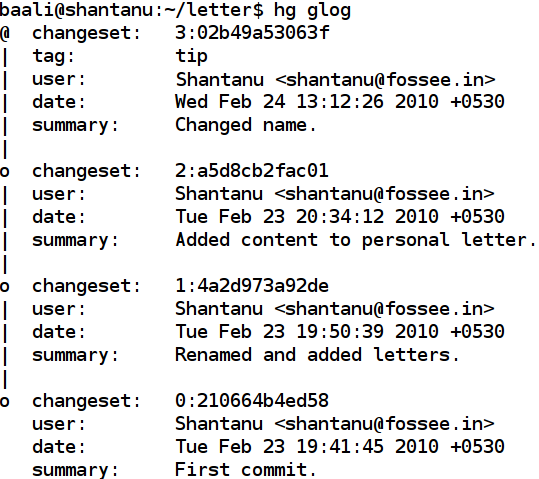
\includegraphics[height=2in, interpolate=true]{glog-main}
    \end{block}
    \column{0.5\textwidth} 
    \begin{block}{\center{cloned directory}}
      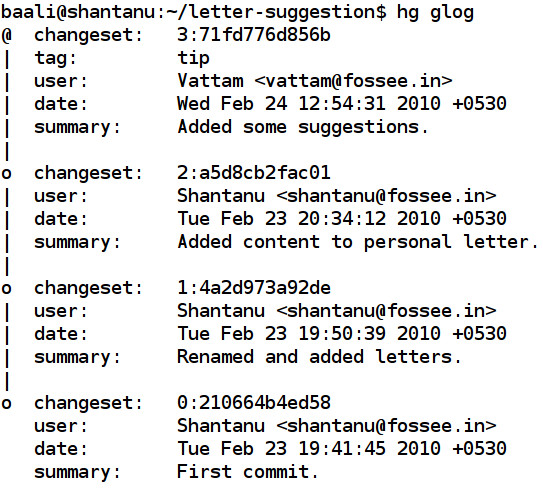
\includegraphics[height=2in, interpolate=true]{glog-suggestion}
    \end{block}
  \end{columns}
\end{frame}

\begin{frame}[fragile]
  \frametitle{Merging}
  \emphbar{Lets sync both these branches!}
  \begin{lstlisting}
$ hg pull ../letter-suggestion
pulling from ../letter-suggestion
searching for changes
adding changesets
adding manifests
adding file changes
added 1 changesets with 1 changes to 1 files (+1 heads)
(run 'hg heads' to see heads, 'hg merge' to merge)    
  \end{lstlisting} %$
  \begin{itemize}
  \item \typ{pull} can be done from a branch explicitly also.
  \pause
  \item \alert{Output is already suggesting something!}
  \end{itemize}  
\end{frame}

%% Here one can mention the point of having push and pull separate. Because of this policy, changes made are not lost.
\begin{frame}[fragile]
  \frametitle{Analyzing events in detail}
  Since hg \typ{pull} don't update the files directly, our changes are still safe. \typ{hg} provides some commands to help understand such problems.
\begin{tiny}
  \begin{lstlisting}
$ hg heads 
changeset:   4:71fd776d856b
tag:         tip
parent:      2:a5d8cb2fac01
user:        Vattam <vattam@fossee.in>
date:        Wed Feb 24 12:54:31 2010 +0530
summary:     Added some suggestions.

changeset:   3:02b49a53063f
user:        Shantanu <Shantanu@fossee.in>
date:        Wed Feb 24 13:12:26 2010 +0530
summary:     Changed name.
  \end{lstlisting} %%$
\end{tiny}
  It shows current repository heads or show branch head
\end{frame}

\begin{frame}[fragile]
  \frametitle{What went wrong: Analysis}
    \begin{lstlisting}
$ hg glog    
  \end{lstlisting} %%$
  \begin{center}
  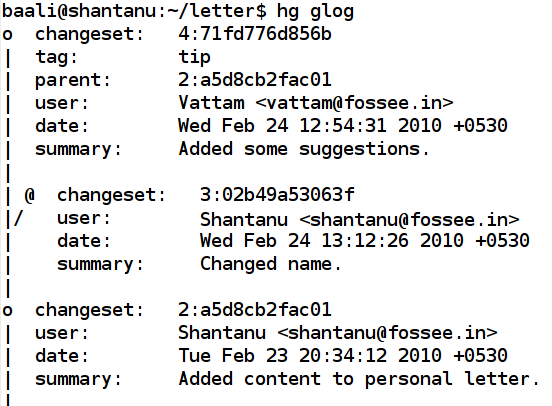
\includegraphics[height=2in]{heads}  
  \end{center}  
  It shows history alongside an ASCII revision graph.  
\end{frame}

\begin{frame}[fragile]
  \frametitle{What went wrong: Analysis cont...}
  Because of different 'pasts', \typ{up} command fails.
  \begin{lstlisting}
$ hg up
abort: crosses branches (use 'hg merge' 
       or 'hg update -C')
  \end{lstlisting} %$
\end{frame}

\begin{frame}[fragile]
  \frametitle{Merging}
  To deal such situations \typ{hg} \alert{merge} command merge working directory with another revision.
  \begin{lstlisting}
$ hg merge
 1 files updated, 0 files merged, 0 files removed, 0 files unresolved
(branch merge, don't forget to commit)   
  \end{lstlisting} %$
  After merging two branches, we have to commit the results to create a common head.
  \begin{lstlisting}
$ hg ci -u "Shantanu <shantanu@fossee.in>" 
        -m "Merged branches."
  \end{lstlisting} %$
  \inctime{15}
\end{frame}

\begin{frame}[fragile]
  \frametitle{\typ{glog}}
  \begin{center}
  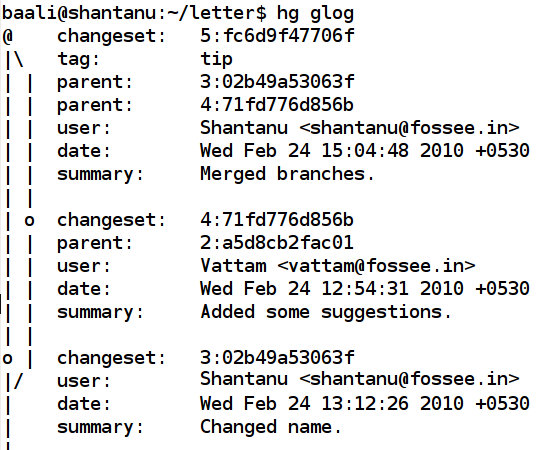
\includegraphics[height=2.8in]{glog-2}  
  \end{center}
\end{frame}

\begin{frame}[fragile]
  \frametitle{Revisiting history!}
  In case earlier girl is available again and you are still looking for date you can \alert{revert} back to previous letter!
  \begin{lstlisting}
$ hg revert -r 2 -a
reverting letter-personal.tex    
  \end{lstlisting} %%$
  And the content changes. From here on you can further change your letter as you wish.
  %% more options for revert are to explained here!
\end{frame}

\begin{frame}[fragile]
  \frametitle{More information}
  \begin{itemize}
  \item \typ{merge} fails if there are conflicting changes.
    \begin{itemize}
    \item Like two persons editing same file, same line and pushing it upstream.
    \end{itemize}
  \item In conflicts, one have to perform \typ{merge} manually.
  \item \typ{hg} provides \alert{\typ{incoming}} command, which checks the would-be imported changes
    \begin{itemize}
    \item To avoid conflicting changes before importing.
    \end{itemize}
  \end{itemize}
  \inctime{10}
\end{frame}

%% Manual and force merge
%% hgignore

%% Reverting to previous versions!
% Steps to follow to make life easier. How to avoid/handle manual merges.
\section{Work flow: DOS and DON'Ts}

\begin{frame}
  \frametitle{Motto behind hg}
  \begin{center}
  \color{red}{``Commit Early Commit Often.''}
  \end{center}  
\end{frame}

\begin{frame}
  \frametitle{Work-flow}
  \begin{itemize}
  \item Make changes.
  \item Commit.
  \item Pull changesets.
  \item Merge(if required).
  \item Push.
  \end{itemize}
\end{frame}

\begin{frame}
  \frametitle{Cheat Sheet}
  \begin{center}
  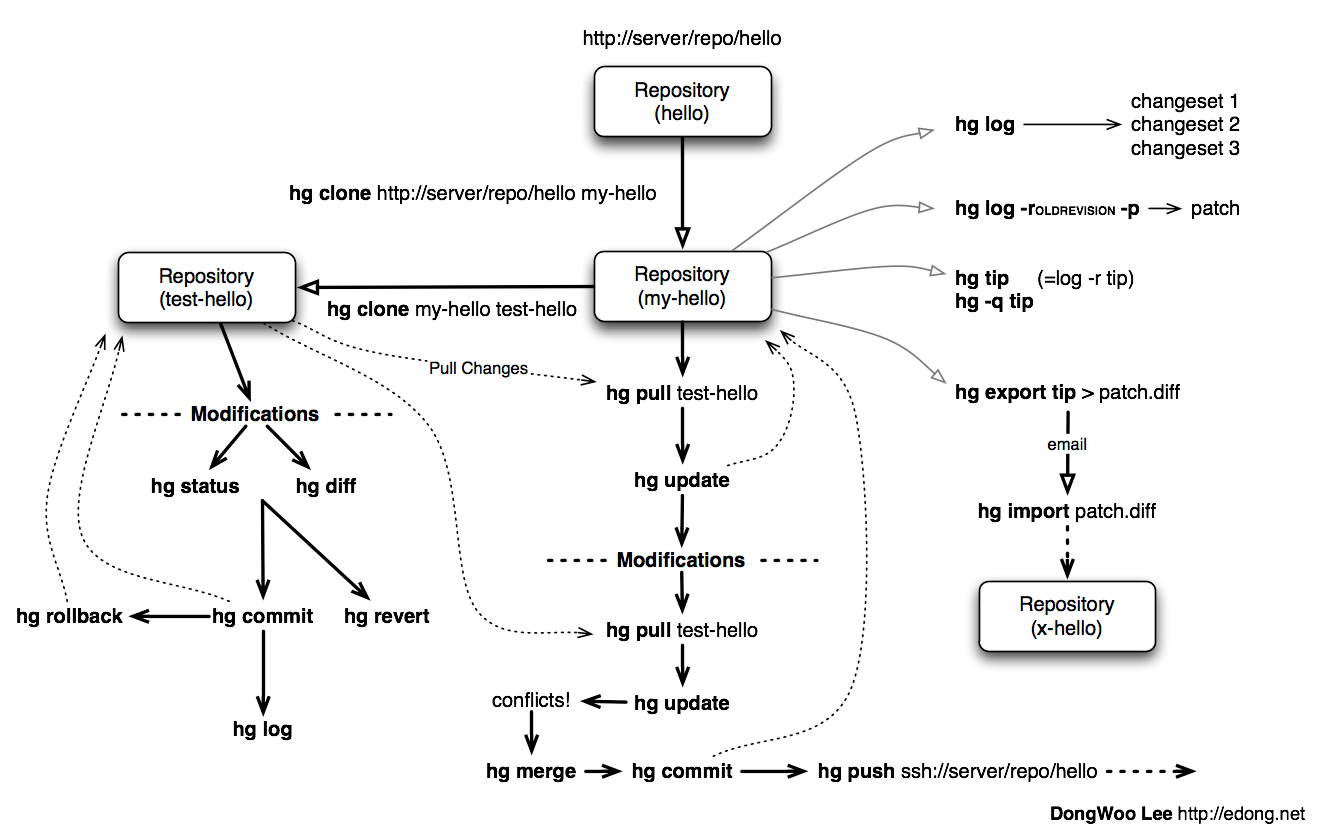
\includegraphics[height=2.8in]{mod}  
  \end{center}  
  \inctime{15}
\end{frame}

%% Move it to end of session. Once introduction part is 
%% over. Then mentioning about options and utility.
\section{Use case and Options}

\begin{frame}
  \frametitle{Use cases}
  \emphbar{For team of people working remotely(even different computers/machines) on a project, use of version control is inevitable!}
  \vspace{0.15in}
  \emphbar{For single person: managing projects and assignments becomes easy}
  \vspace{0.15in}
  \pause
  \emphbar{\color{red}{It is a good habit!}}
\end{frame}

\begin{frame}
  \frametitle{What are other options!}
  \begin{itemize}
  \item cvs (Concurrent Version System)
  \item svn (Subversion)
  \item hg (Mercurial)
  \item bzr (Bazaar)
  \item git
  \end{itemize}
  \inctime{5}
\end{frame}

\begin{frame}
  \frametitle{Suggested Readings:}
  \begin{itemize}
  \item \url{http://mercurial.selenic.com/guide/}
  \item \url{http://hgbook.red-bean.com/}    
  \item \url{http://karlagius.com/2009/01/09/version-control-for-the-masses/}
  \item Articles related to version control available on \url{http://betterexplained.com/}
  \item \url{http://en.wikipedia.org/wiki/Revision_control}
  \item \url{http://wiki.alliedmods.net/Mercurial_Tutorial}
  \item Mario game images are taken from wikipedia.
  \end{itemize}
\end{frame}
\end{document}

Some more suggestions from Nishanth:
revert  
resolve

Notes
-----

From http://mercurial.selenic.com/

Quick Start

Clone a project and push changes

$ hg clone http://selenic.com/repo/hello
$ cd hello
$ (edit files)
$ hg add (new files)
$ hg commit -m 'My changes'
$ hg push


Create a project and commit

$ hg init (project-directory)
$ cd (project-directory)
$ (add some files)
$ hg add
$ hg commit -m 'Initial commit'
